\begin{frame}{Semi-Lagrangian Scheme}
    \textbf{The Semi-Lagrangian scheme is defined as it follows:}
    \centering
    \begin{equation*}
        u\left(t_{n+1}, x_i\right)=\mathcal{I}_h^m\left(u\left(t_n, x\right)\right)\left(x_i-a \Delta t\right)
    \end{equation*}
    \begin{figure}
        \centering
        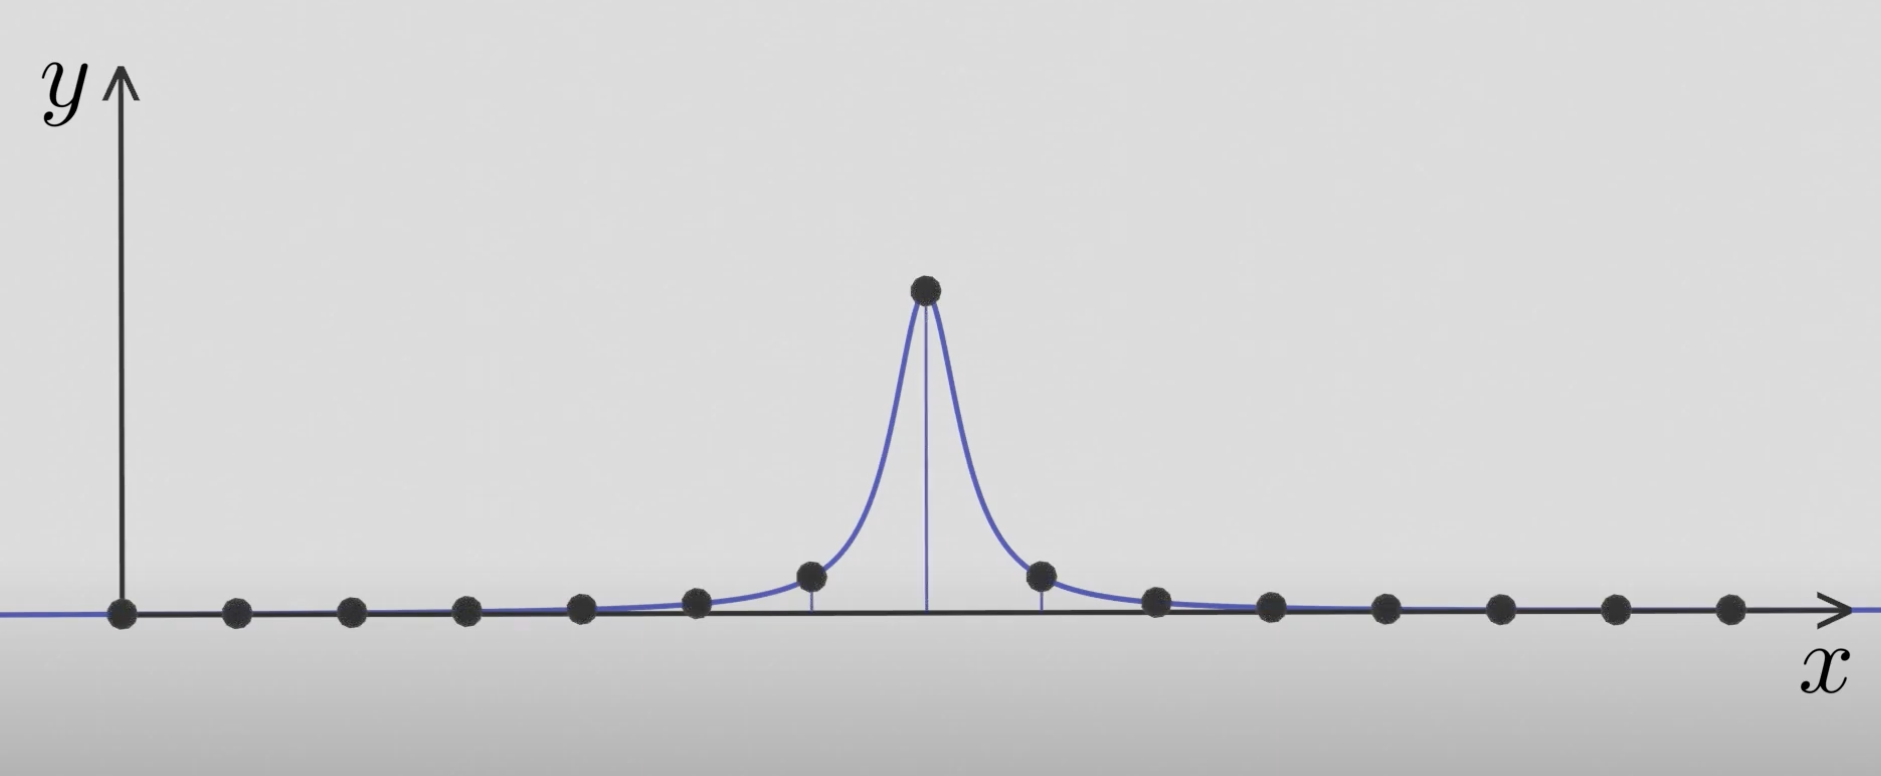
\includegraphics[width=0.3\textwidth]{images/semil1.png}
        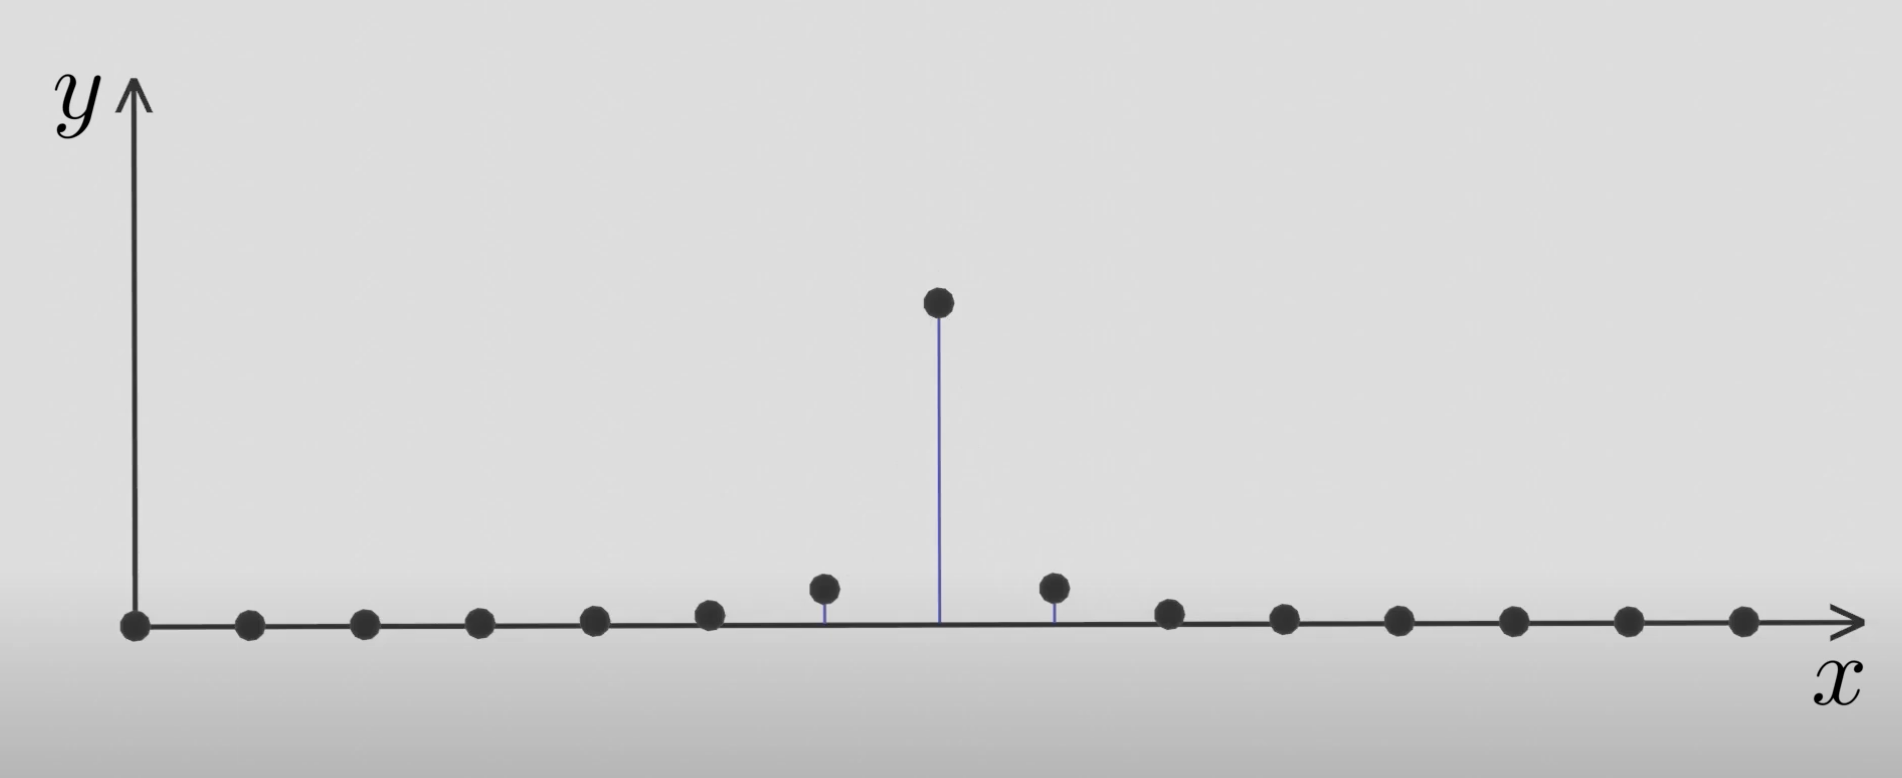
\includegraphics[width=0.3\textwidth]{images/semil2.png}
        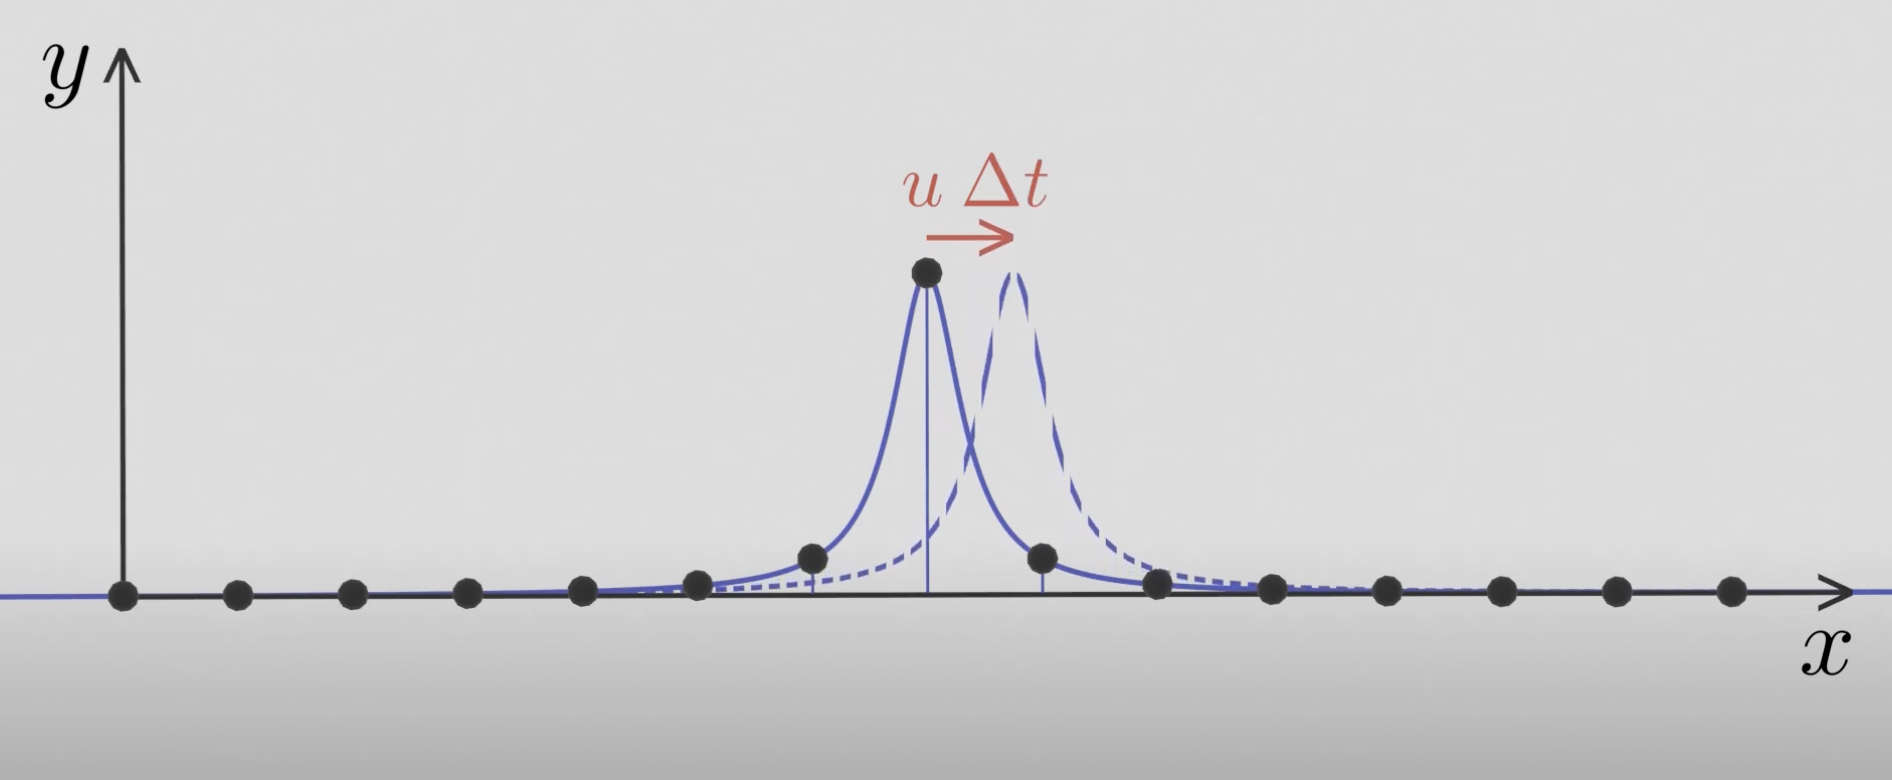
\includegraphics[width=0.3\textwidth]{images/semil2.1.png}
        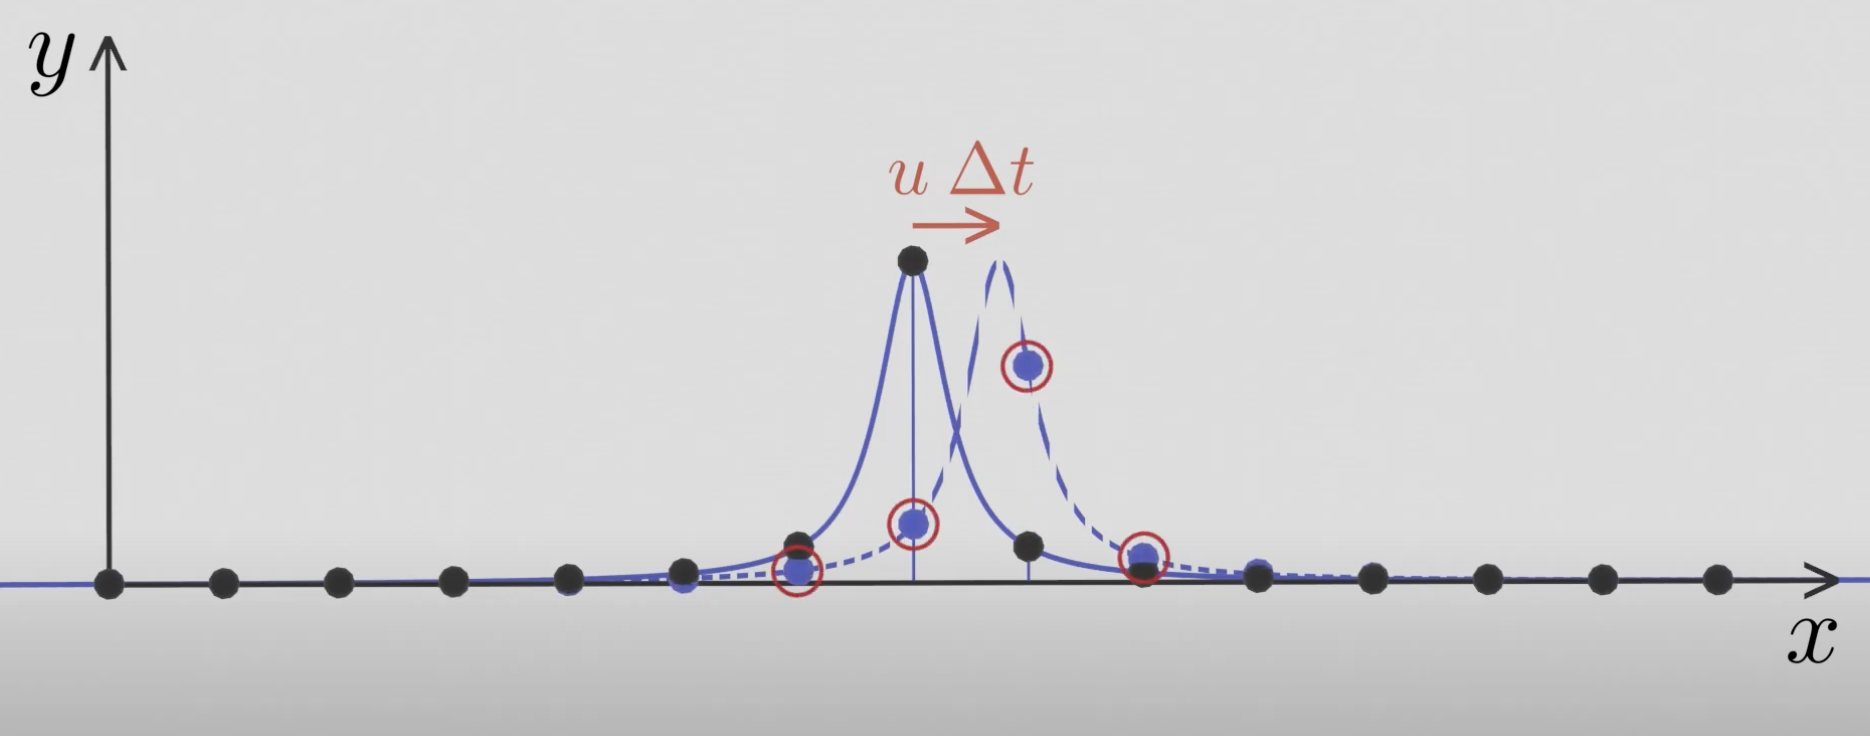
\includegraphics[width=0.3\textwidth]{images/semil3.png}
        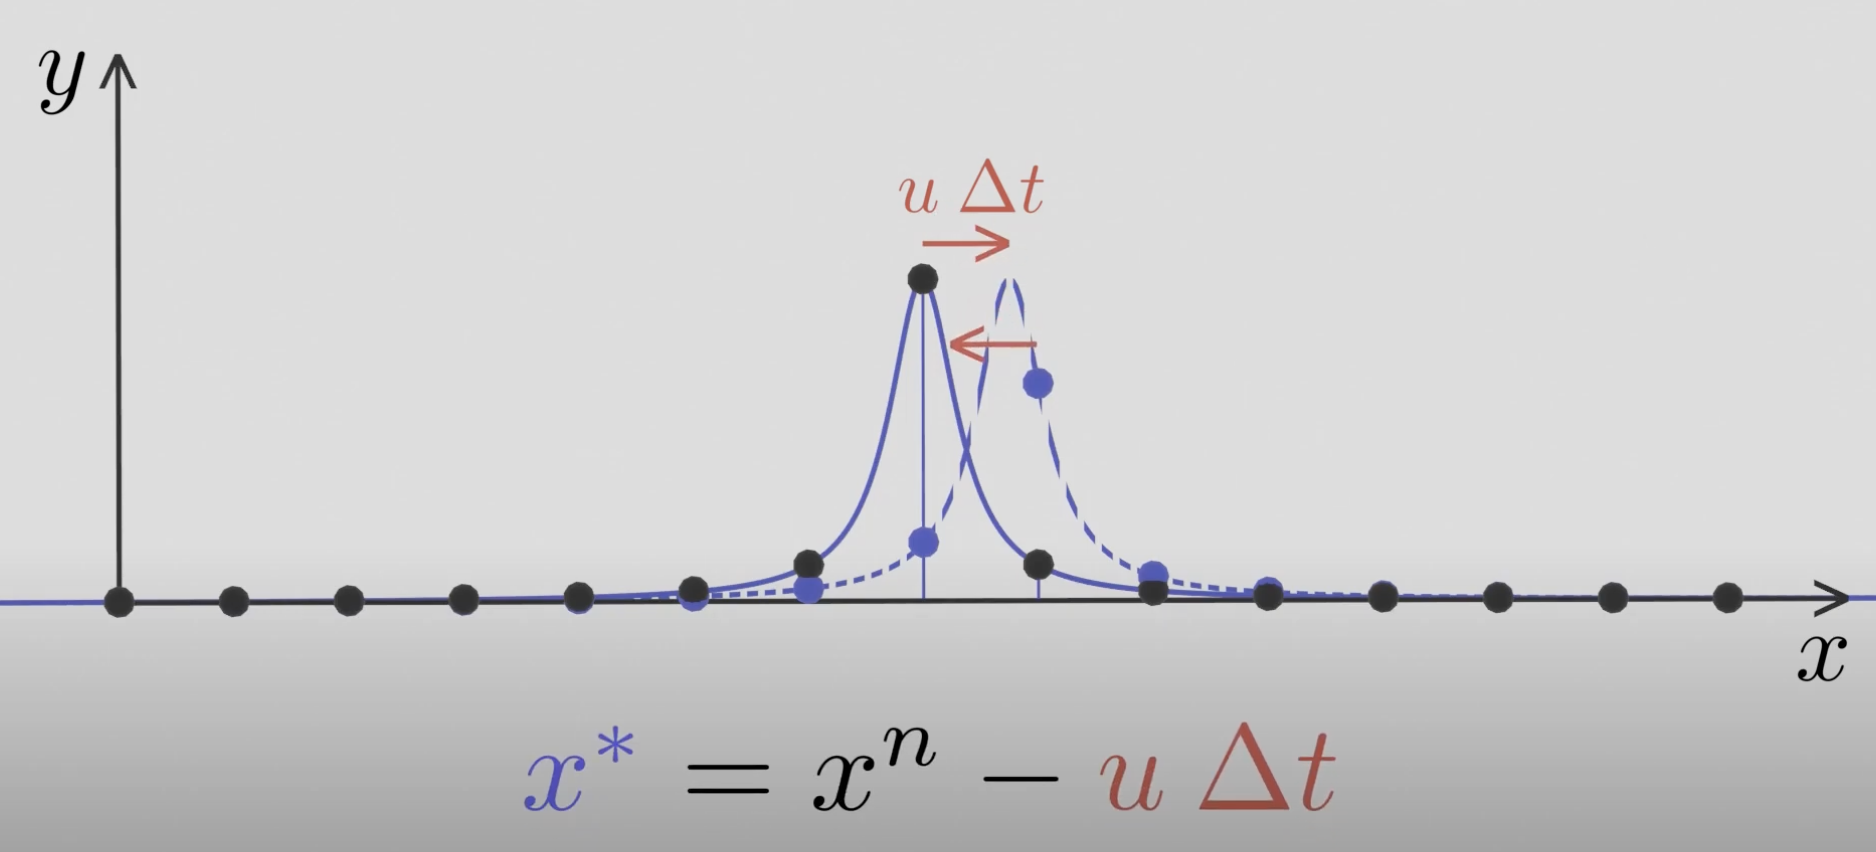
\includegraphics[width=0.3\textwidth]{images/semil4.png}
        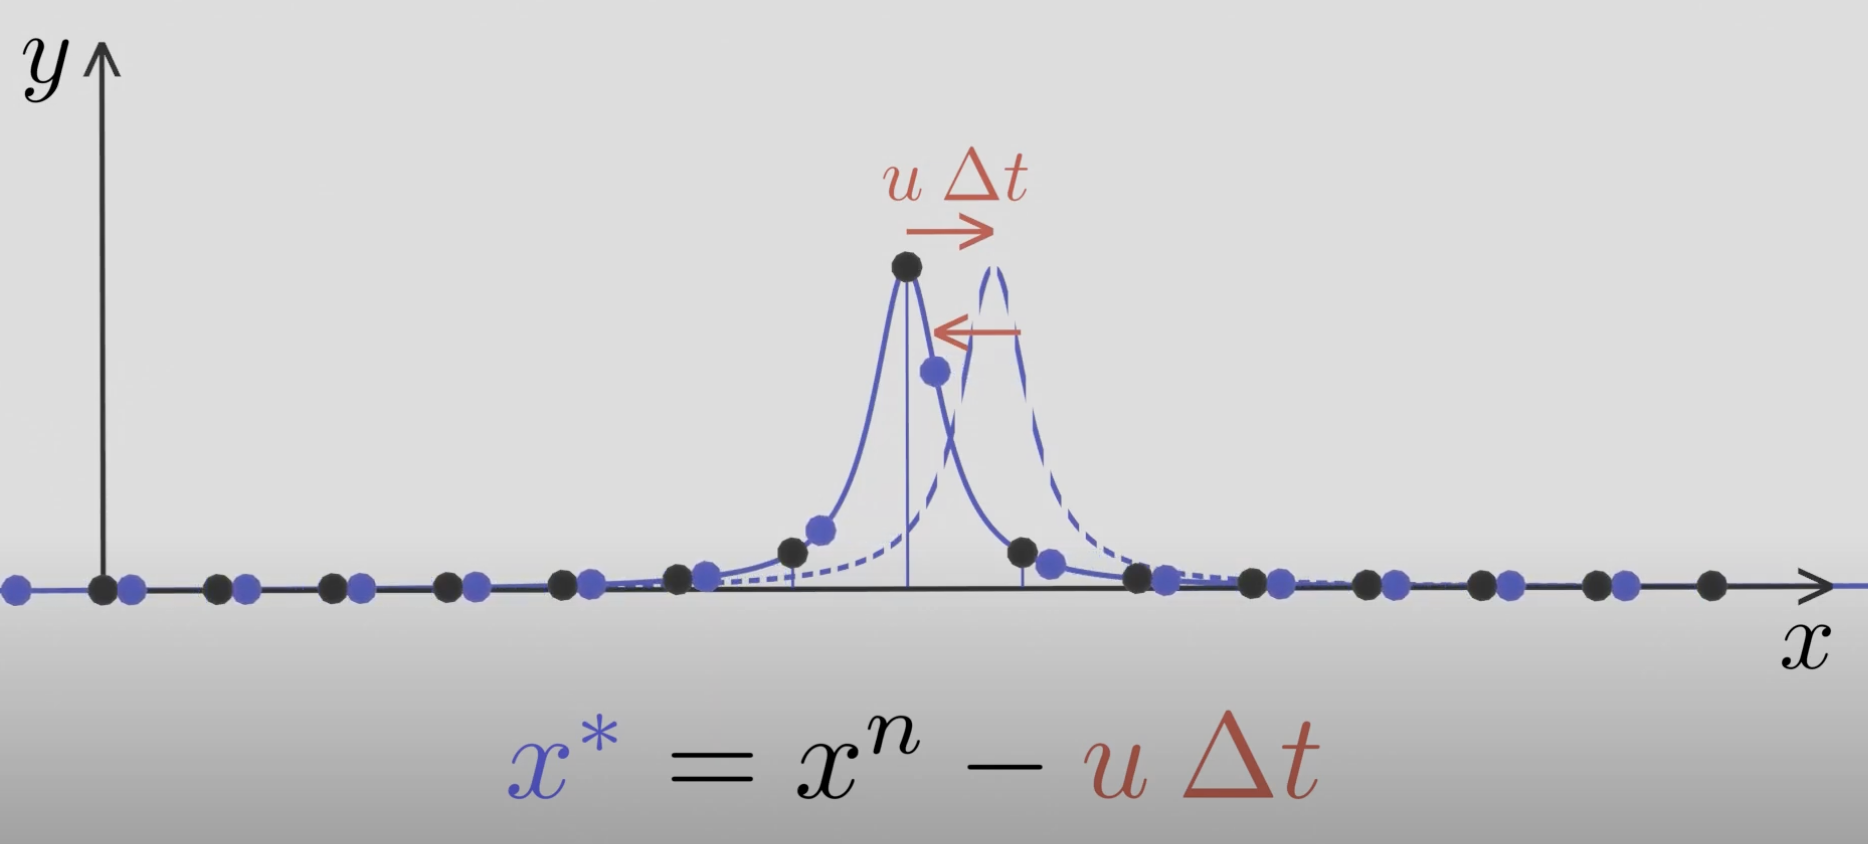
\includegraphics[width=0.3\textwidth]{images/semil5.png}
        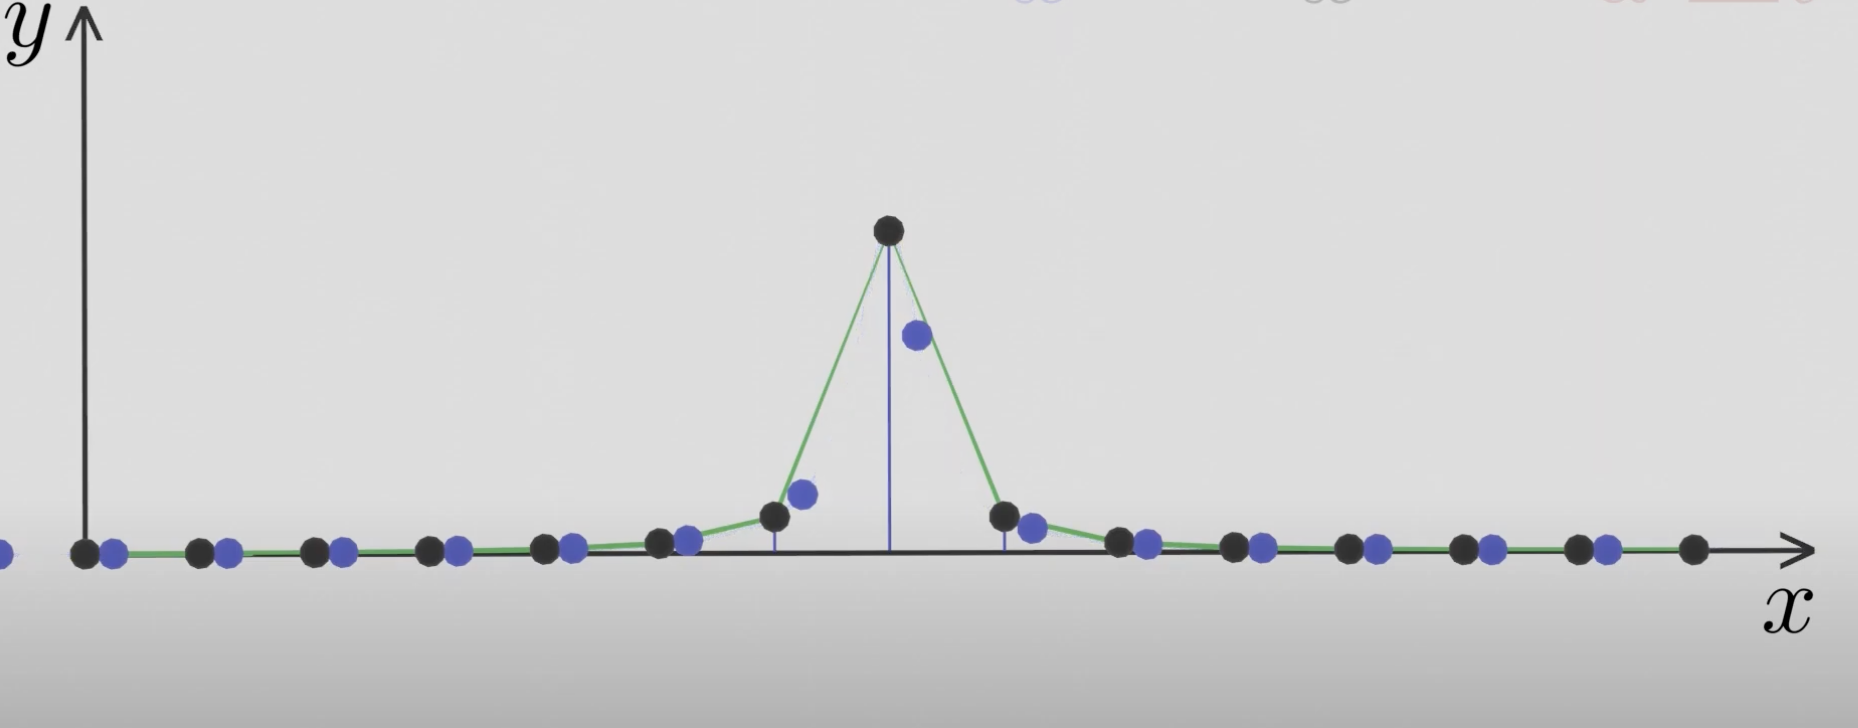
\includegraphics[width=0.3\textwidth]{images/semil6.png}
        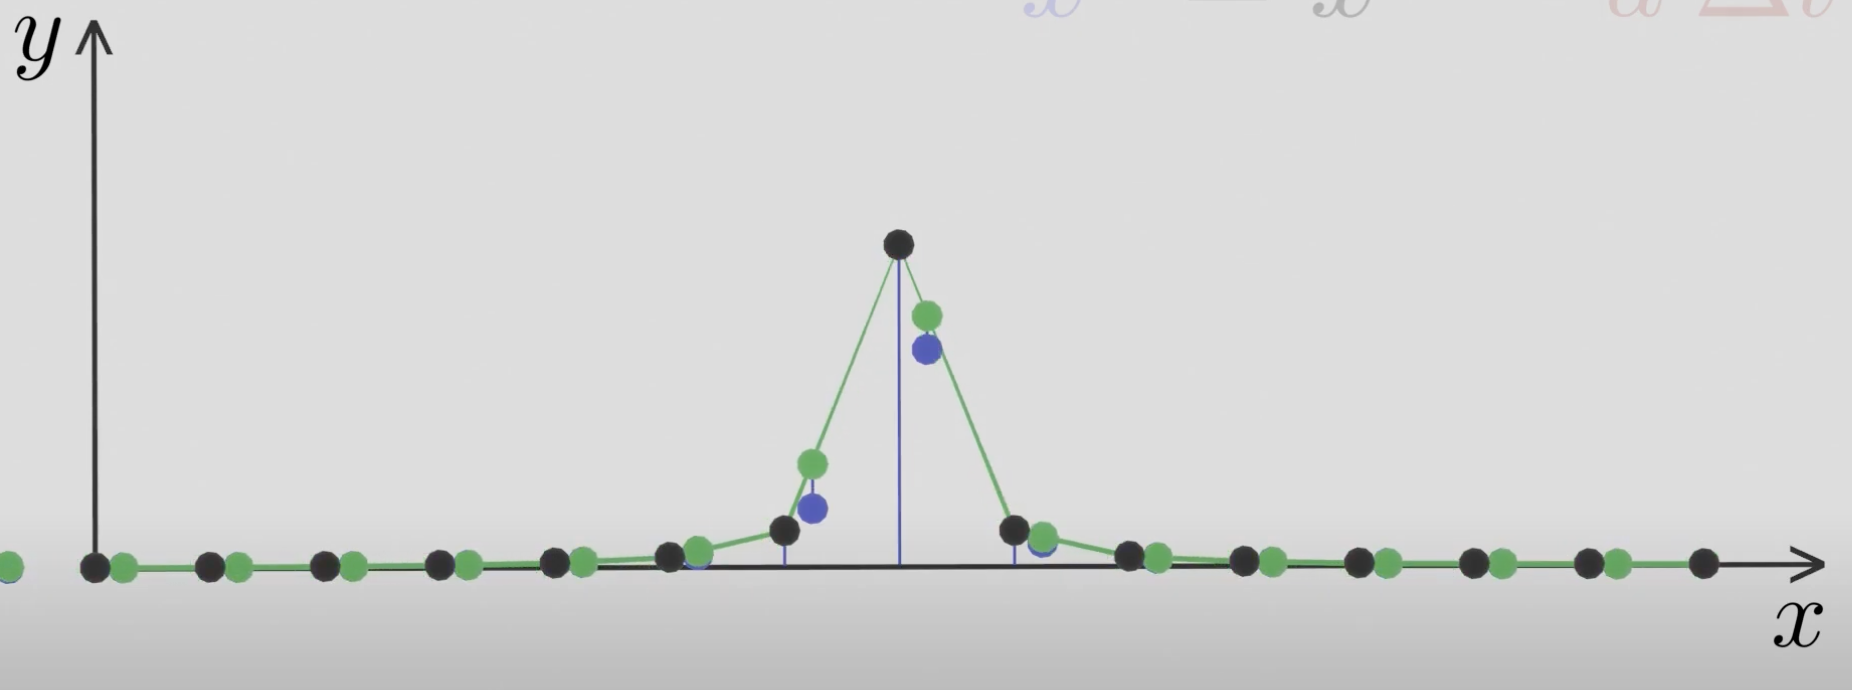
\includegraphics[width=0.3\textwidth]{images/semil7.png}
        \caption{Semi-Lagrangian Scheme}
    \end{figure}

\end{frame}
